\documentclass{article}
\usepackage[english,russian]{babel}
\usepackage{textcomp}
\usepackage{geometry}
  \geometry{left=2cm}
  \geometry{right=1.5cm}
  \geometry{top=1.5cm}
  \geometry{bottom=2cm}
\usepackage{tikz}
\usepackage{multicol}
\usepackage{hyperref}
\usepackage{listings}
\usepackage{pmboxdraw}
\usepackage{fancyvrb}
\pagenumbering{gobble}

\lstdefinestyle{csMiptCppStyle}{
  language=C++,
  basicstyle=\linespread{1.1}\ttfamily,
  columns=fixed,
  fontadjust=true,
  basewidth=0.5em,
  keywordstyle=\color{blue}\bfseries,
  commentstyle=\color{gray},
  texcl=true,
  stringstyle=\ttfamily\color{orange!50!black},
  showstringspaces=false,
  numbersep=5pt,
  numberstyle=\tiny\color{black},
  numberfirstline=true,
  stepnumber=1,      
  numbersep=10pt,
  backgroundcolor=\color{white},
  showstringspaces=false,
  captionpos=b,
  breaklines=true
  breakatwhitespace=true,
  xleftmargin=.2in,
  extendedchars=\true,
  keepspaces = true,
  tabsize=4,
  upquote=true,
}


\lstdefinestyle{csMiptCppLinesStyle}{
  style=csMiptCppStyle,
  frame=lines,
}

\lstdefinestyle{csMiptCppBorderStyle}{
  style=csMiptCppStyle,
  framexleftmargin=5mm, 
  frame=shadowbox, 
  rulesepcolor=\color{gray}
}


\lstdefinestyle{csMiptBash}{
  	style=csMiptCppStyle,
	breaklines=true,
	frame=tb,
	language=bash,
	breakatwhitespace=true,
	alsoletter={*()"'0123456789.},
	alsoother={\{\=\}},
	basicstyle={\ttfamily},
	keywordstyle={\bfseries},
	literate={{=}{{{=}}}1},
	prebreak={\textbackslash},
	sensitive=true,
	stepnumber=1,
	tabsize=4,
	morekeywords={echo, function},
	otherkeywords={-, \{, \}},
	literate={\$\{}{{{{\bfseries{}\$\{}}}}2,
	upquote=true,
	frame=none
}

\lstset{style=csMiptCppStyle}
\lstset{
        literate={~}{{\raisebox{0.5ex}{\texttildelow}}}{1}
}


\renewcommand{\thesubsection}{\arabic{subsection}}
\makeatletter
\def\@seccntformat#1{\@ifundefined{#1@cntformat}%
   {\csname the#1\endcsname\quad}
   {\csname #1@cntformat\endcsname}}
\newcommand\section@cntformat{}     
\newcommand\subsection@cntformat{Задача \thesubsection.\space} 
\newcommand\subsubsection@cntformat{\thesubsubsection.\space}
\makeatother



\begin{document}
\title{Семинар \#2: git, продолжение. Практика. \vspace{-5ex}}\date{}\maketitle
Для сдачи этого и будущих ДЗ вам нужно создать репозиторий на GitLab (если он ещё не создан) под названием \texttt{devtools-homework}. Структура репозитория должна иметь вид:
\begin{center}
\begin{BVerbatim}
├── seminar2_more_git/
│   ├── 01.sh
│   ├── 02.sh
│   └── ...
└── ...
\end{BVerbatim}
\end{center}



\subsection*{Подготовка. Генерация репозитория, который будет использоваться в задачах.}
Для решения следующих задач вам потребуется создать простой репозиторий, состоящий из четырёх коммитов, с помощью bash-скрипта. Для этого сделайте следующее:
\begin{enumerate}
\item Зайдите в репозиторий \href{https://mipt-hsse.gitlab.yandexcloud.net/v.biryukov/devtools_course}{\texttt{mipt-hsse.gitlab.yandexcloud.net/v.biryukov/devtools\_course}}, пройти в папку\\ 
\texttt{seminar2\_git\_advanced/practice}, открыть файл \texttt{create\_animals.sh} и скачать его.

\item Скопируйте скрипт в папку, в которой вы будете его запускать. Убедитесь, что папка, куда вы копируете скрипт не является частью другого репозитория, а также не содержит внутри себя папку \texttt{animals}.

\item Откройте терминал и зайти в папку, содержащую скрипт
\begin{lstlisting}
$ cd 
\end{lstlisting}

\item Добавьте скрипту права на исполнение
\begin{lstlisting}[style=csMiptBash]
$ chmod +x create_animals.sh
\end{lstlisting}

\item Запустите скрипт, он создаст папку \texttt{animals} с репозиторием внутри
\begin{lstlisting}[style=csMiptBash]
$ ./create_animals.sh
\end{lstlisting}

\item Перейдите в папку \texttt{animals} и убедитесь, что репозиторий создался корректно, напечатав дерево его коммитов:
\begin{lstlisting}[style=csMiptBash]
$ cd animals
$ git log --oneline --graph --all
\end{lstlisting}
\end{enumerate}

\begin{center}
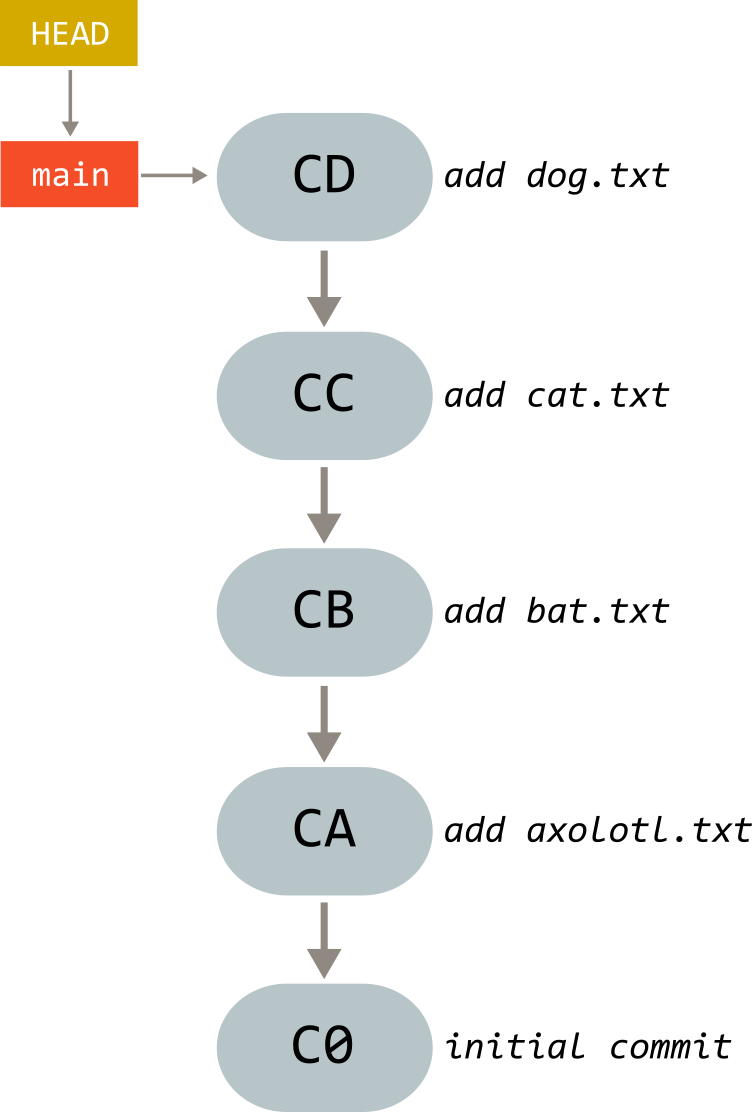
\includegraphics[scale=0.9]{../images/animals.png}
\end{center}



\subsection{Отмена индексации}
Предположим, что вы создали новый файл и добавили его в область индексирования.
\begin{lstlisting}[style=csMiptBash]
$ touch emu.txt
$ git add emu.txt
\end{lstlisting}
Однако затем передумали и хотите убрать этот файл из области индексирования.
Выполните команду, которая бы убирала этот файл из области индексирования, но оставляла бы файл в рабочей папке. Добавлять новые коммиты в этой задаче нельзя.

\subsection{Отмена коммита}
Предположим, что вы создали новый файл и добавили его в область индексирования и в локальный репозиторий.
\begin{lstlisting}[style=csMiptBash]
$ touch emu.txt
$ git add emu.txt
$ git commit -m "add emu.txt"
\end{lstlisting}
Однако затем передумали и хотите отменить коммит. При этом вы хотите, чтобы файл \texttt{emu.txt} продолжал находиться и в рабочей папке и в области индексирования. Выполните команду, которая отменит коммит, оставив рабочую папку и область индексирования неизменными.

\subsection{Отмена \texttt{reset}}
Предположим, что вы решили удалить все коммиты, кроме первого и, находясь на коммите \texttt{CD} (\textit{add dog}) выполнили:
\begin{lstlisting}
$ git reset --hard HEAD~4
\end{lstlisting}
Но потом передумали, и решили вернуть всё обратно. Что для этого нужно сделать?


\subsection{Обратить коммиты}
В этом задании вам нужно обратить коммиты как это показано на изображении. При этом создавать файлы вручную нельзя, можно только использовать команды \texttt{git}.
\begin{center}
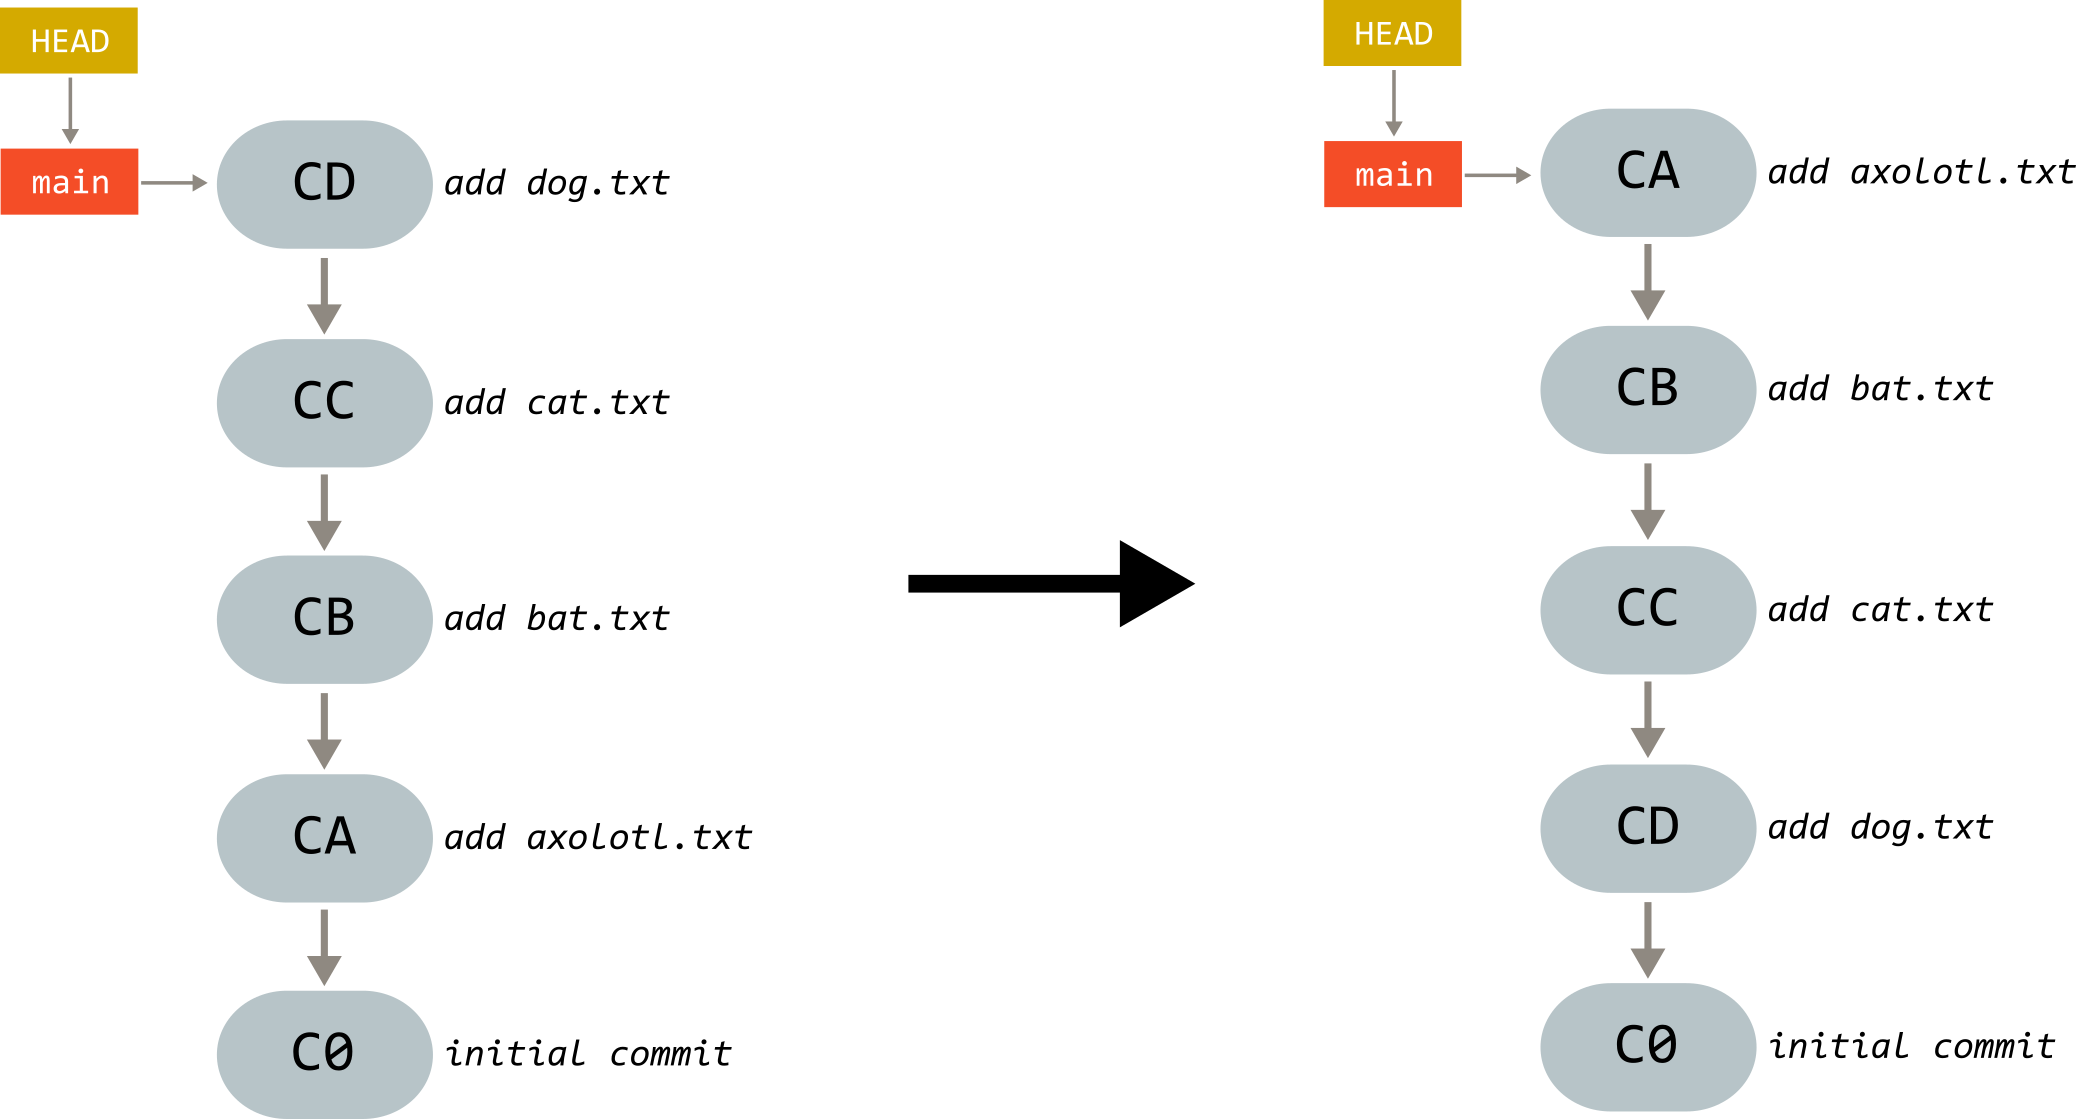
\includegraphics[scale=0.8]{../images/reverse_animals.png}
\end{center}
Решите эту задачу двумя способами:
\begin{enumerate}
\item Создав новую ветку на начальном коммите и добавляя коммиты с помощью \texttt{git cherry-pick}. После этого нужно будет удалить старую ветку и переименовать новую.
\item Используя интерактивное перебазирование.
\end{enumerate}

\subsection{Объединить коммиты}
Пересоздайте репозиторий с помощью скрипта \texttt{create\_animals.sh}.
В этом задании вам нужно объединить все коммиты в один как это показано на изображении. При этом создавать файлы вручную нельзя, можно только использовать команды \texttt{git}.
\begin{center}
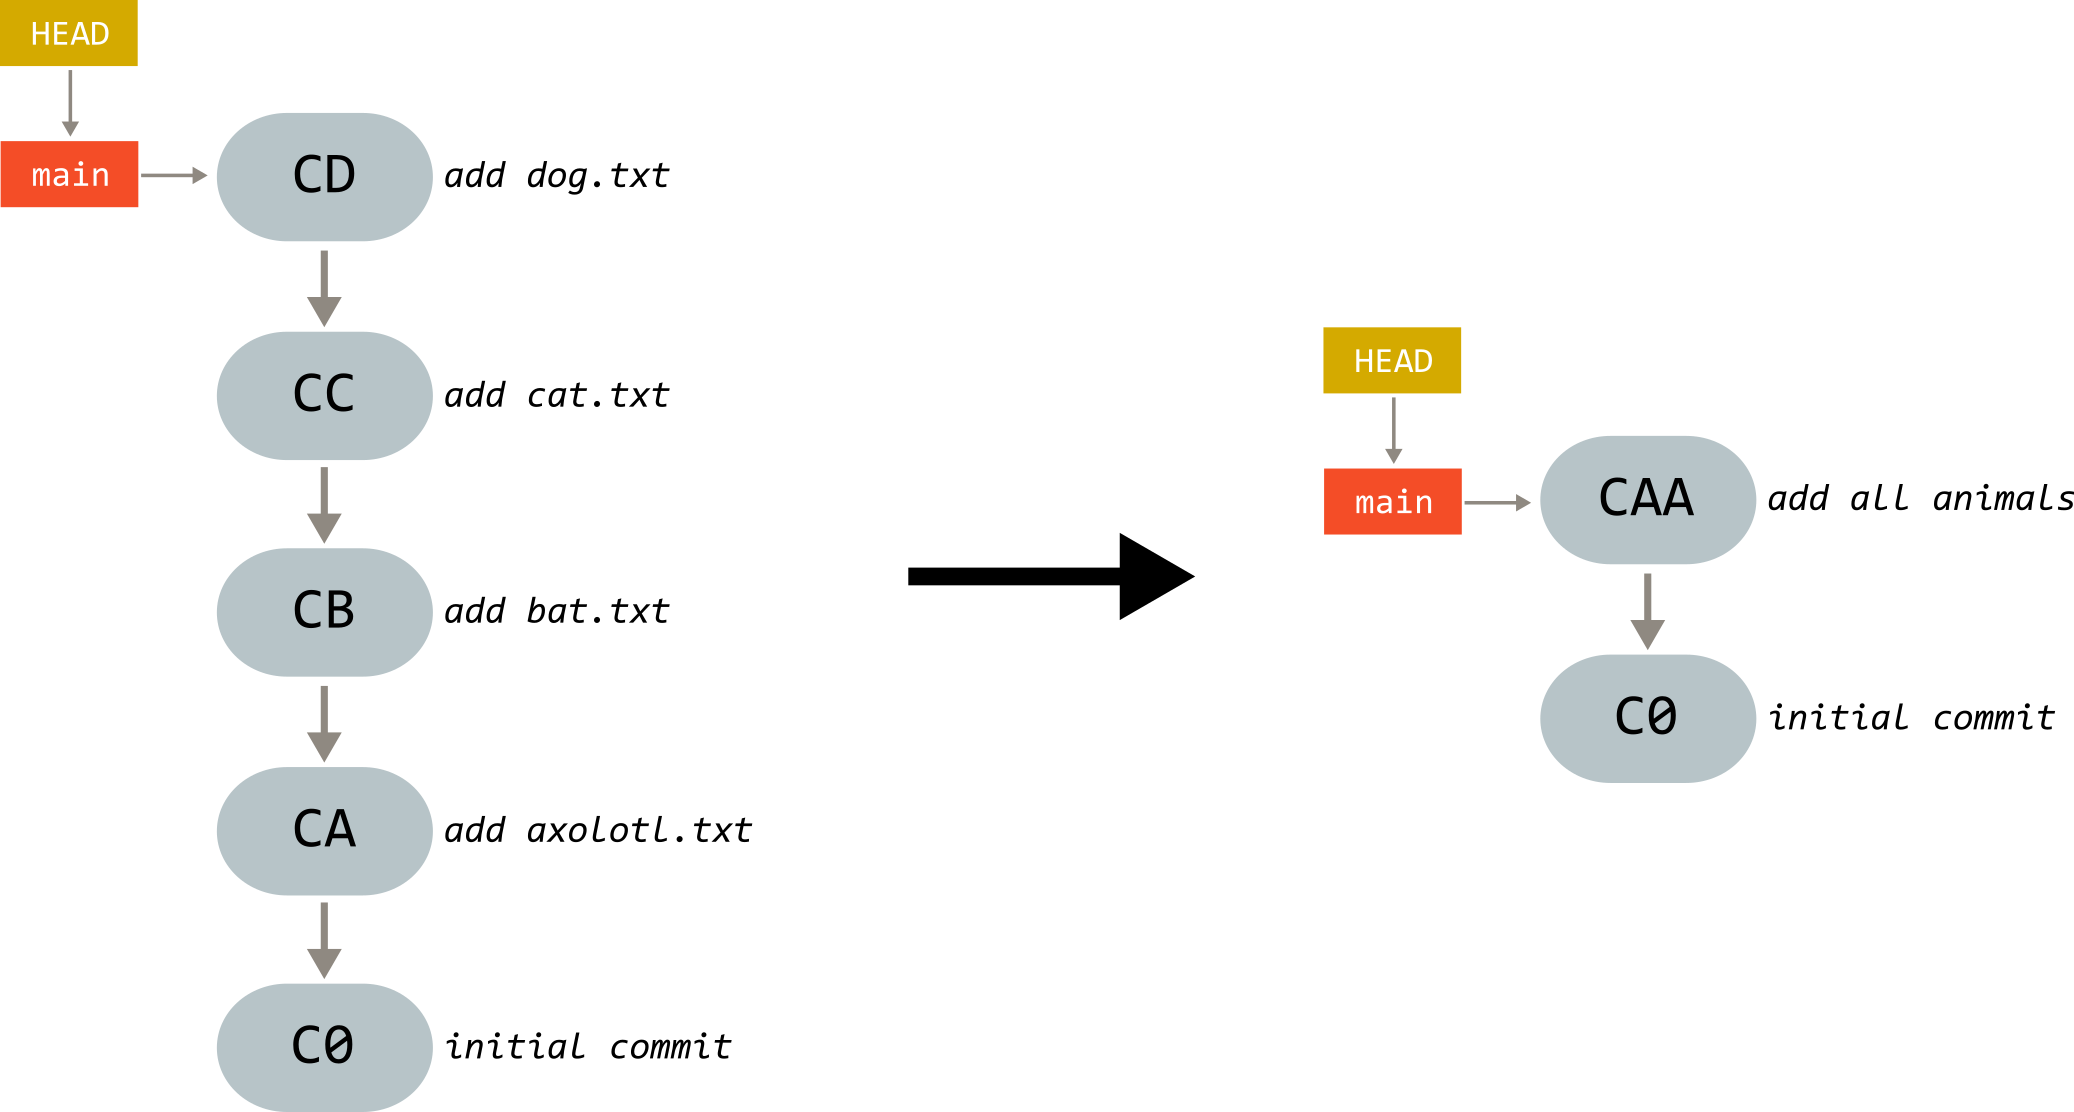
\includegraphics[scale=0.8]{../images/squash_animals.png}
\end{center}
Решите эту задачу двумя способами:
\begin{enumerate}
\item Используя \texttt{reset}.
\item Используя интерактивное перебазирование.
\end{enumerate}

\subsection{Удалить коммиты}
Пересоздайте репозиторий с помощью скрипта \texttt{create\_animals.sh}.
В этом задании вам нужно удалить два коммита, как это показано на изображении. При этом создавать или удалять файлы вручную нельзя, можно только использовать команды \texttt{git}.
\begin{center}
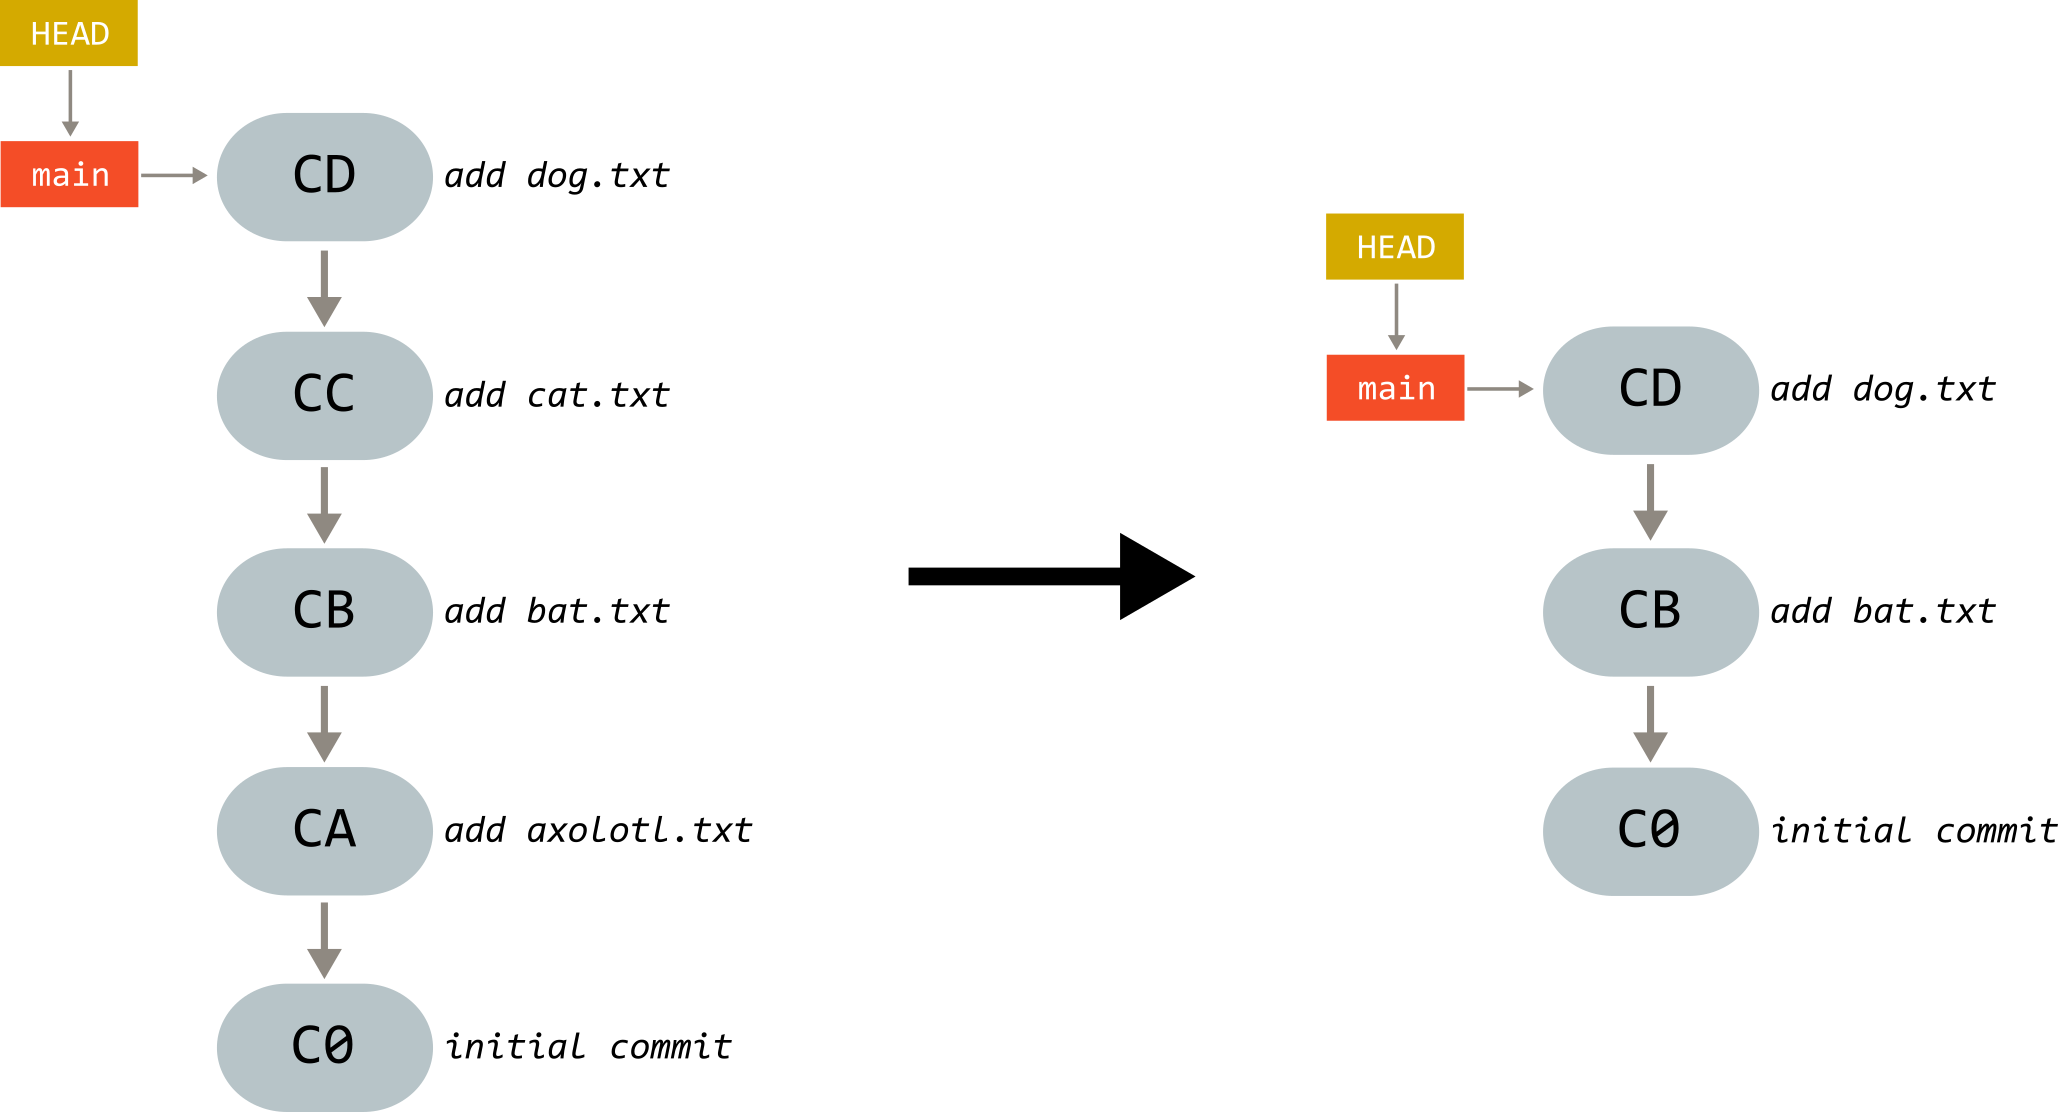
\includegraphics[scale=0.8]{../images/delete_commits_animals.png}
\end{center}
Решите эту задачу двумя способами:
\begin{enumerate}
\item Используя \texttt{cherry-pick}.
\item Используя интерактивное перебазирование.
\end{enumerate}

\subsection{Перераспределить коммиты}
Пересоздайте репозиторий с помощью скрипта \texttt{create\_animals.sh}. В этом задании вам нужно перераспределить коммиты в новые ветки, как это показано на изображении. При этом создавать или удалять файлы вручную нельзя, можно только использовать команды \texttt{git}.
\begin{center}
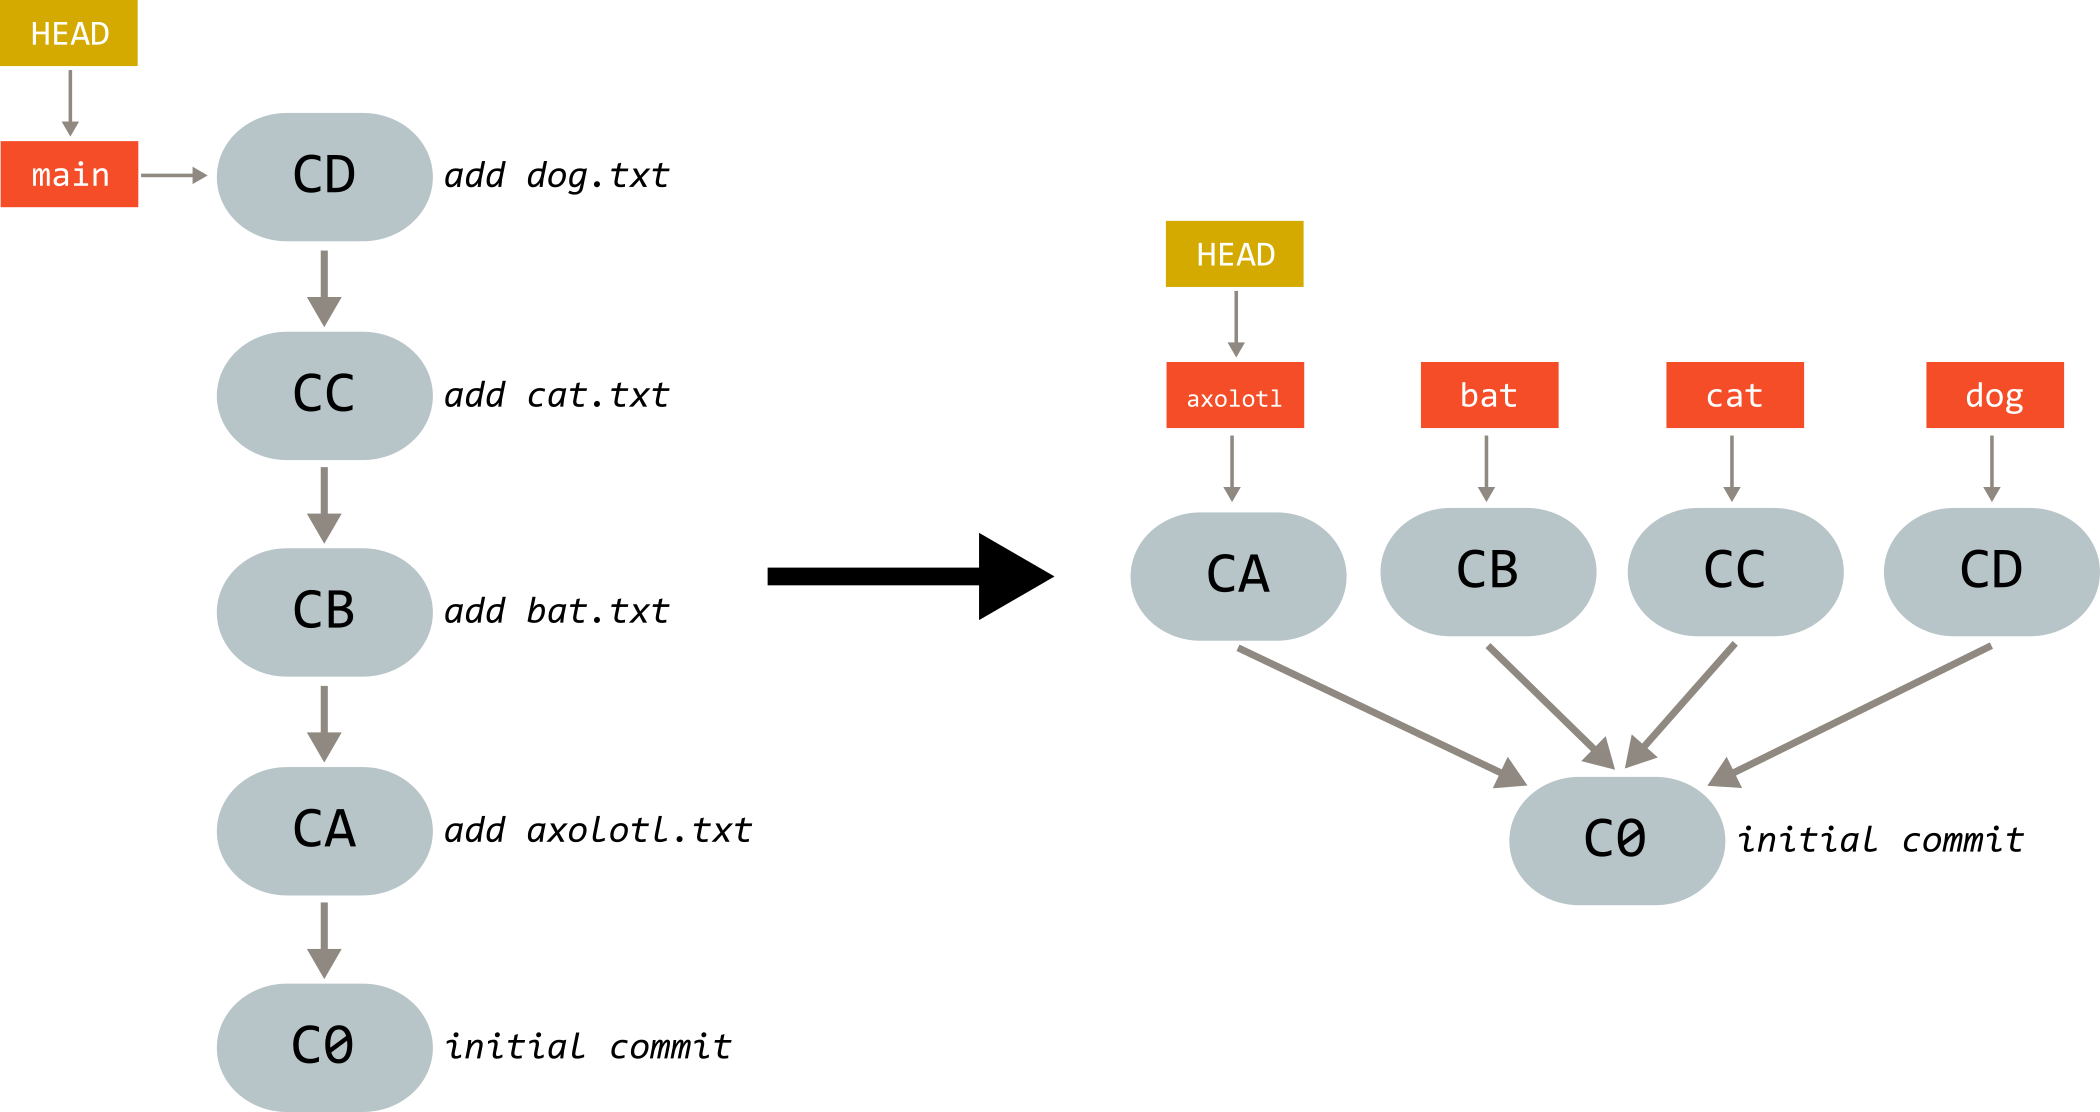
\includegraphics[scale=0.8]{../images/rearrange_animals.png}
\end{center}


\subsection{Отмена слияния}
Создайте новый репозиторий с помощью скрипта \texttt{create\_branch\_animals.sh}. В этом репозитории есть 2 ветки: \texttt{main} и \texttt{other}. Предположим, что вы сделали слияние с помощью команд:
\begin{lstlisting}[style=csMiptBash]
$ git switch main
$ git merge other -m "CM: merging"
\end{lstlisting}

\begin{center}
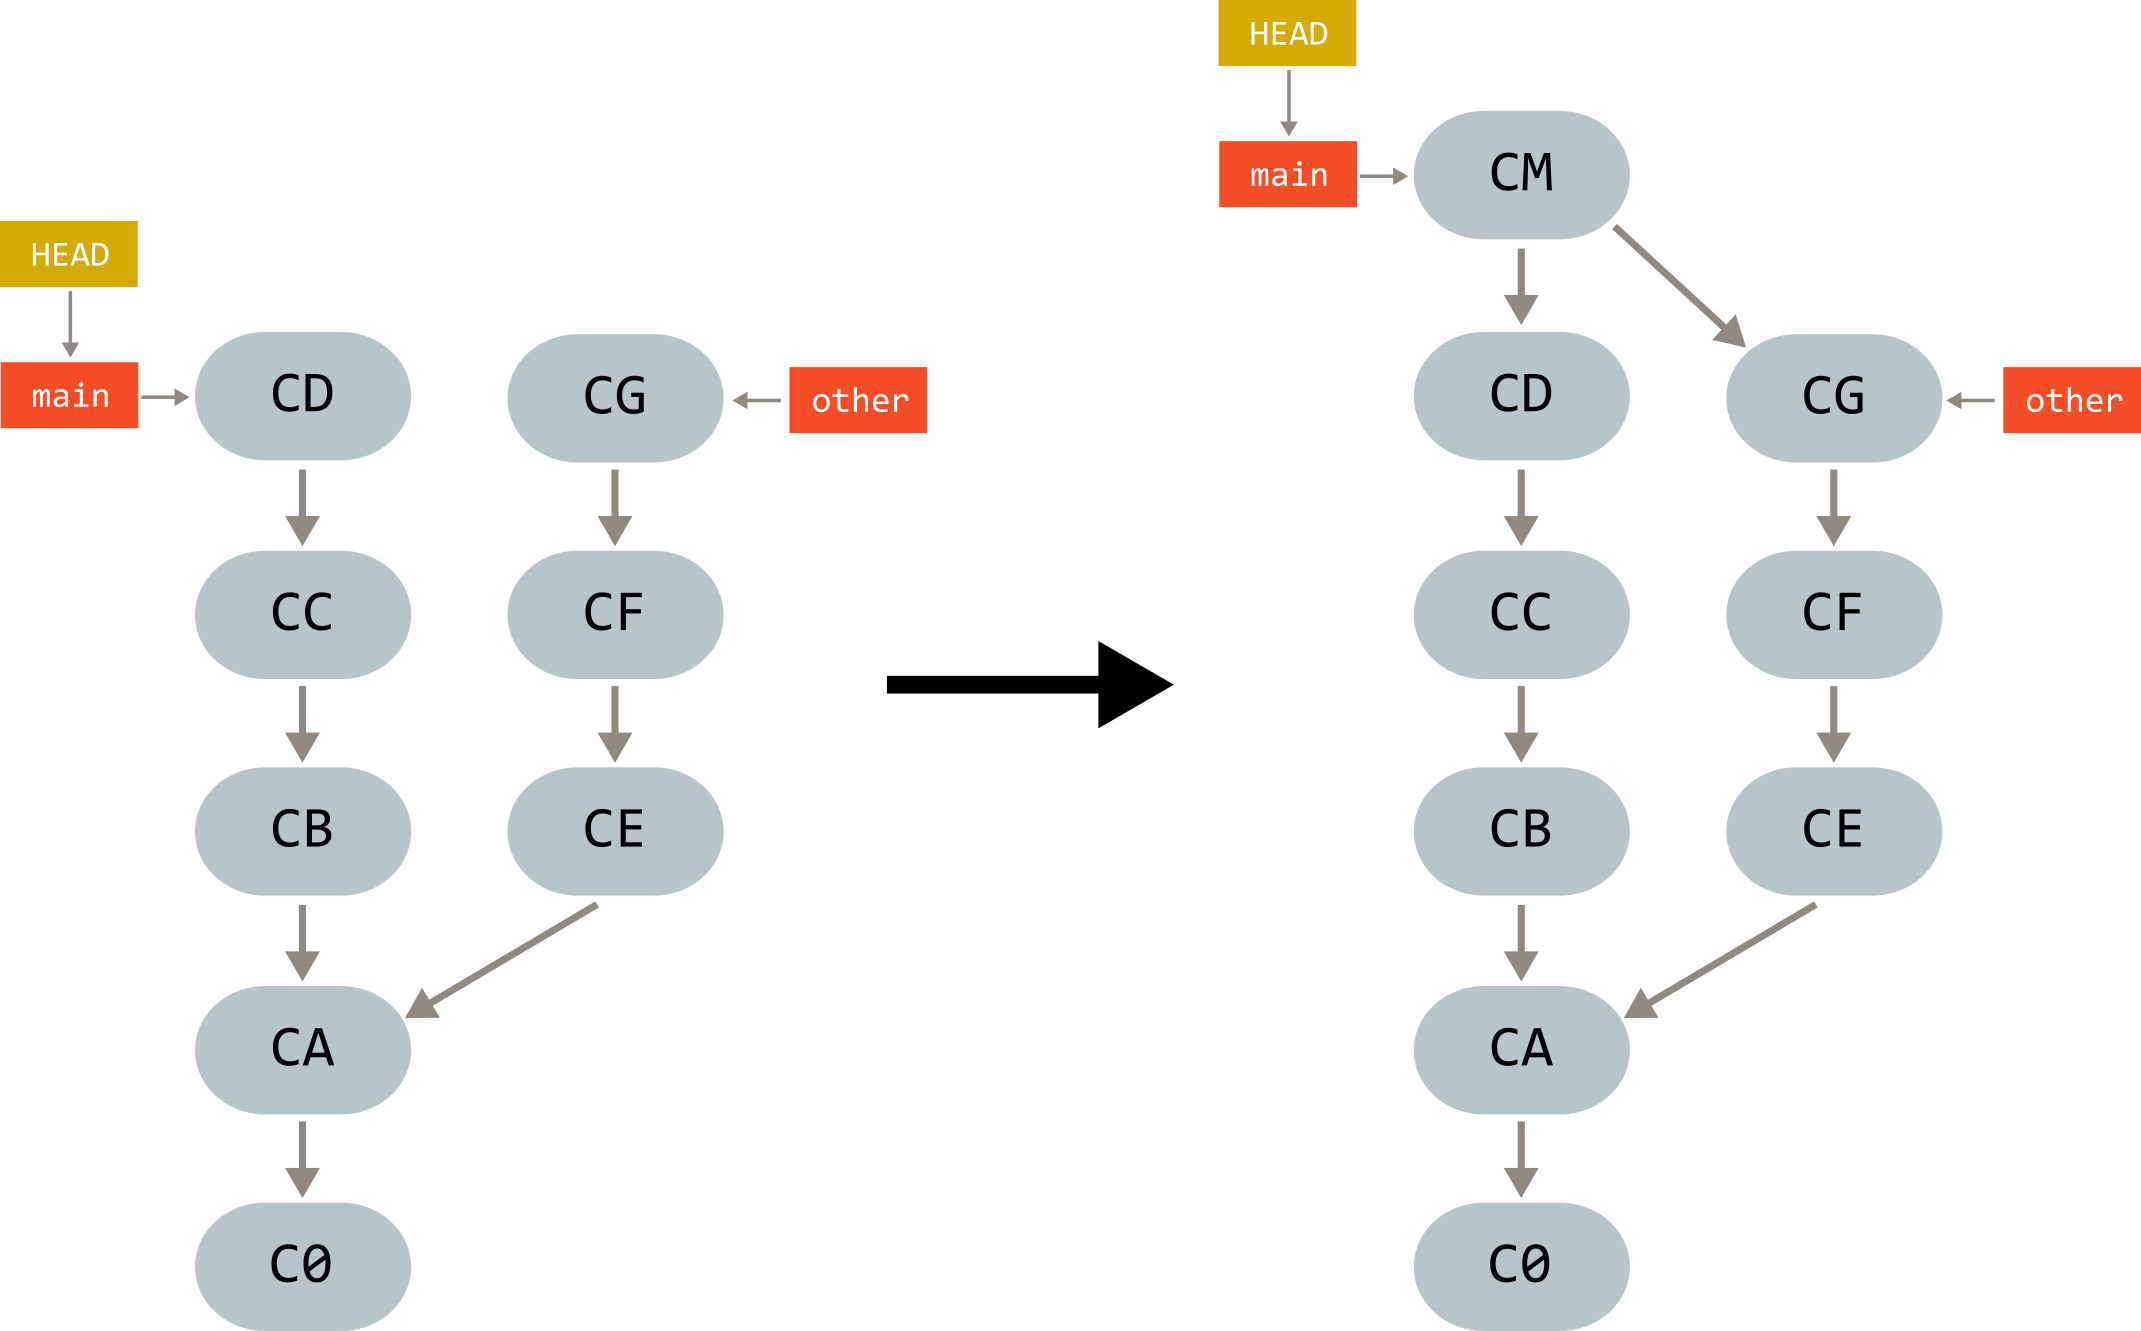
\includegraphics[scale=0.8]{../images/branch_animals_merge.png}
\end{center}

\noindent Однако потом передумали и хотите отменить слияние. Напишите команды \texttt{git}, которые бы отменяли слияние и возвращали бы всё как прежде.


\subsection{Отмена перебазирования}
Создайте новый репозиторий с помощью скрипта \texttt{create\_branch\_animals.sh}. В этом репозитории есть 2 ветки: \texttt{main} и \texttt{other}. Предположим, что вы сделали перебазирование ветки \texttt{other} на ветку \texttt{main} с помощью команд:
\begin{lstlisting}[style=csMiptBash]
$ git switch other
$ git rebase main
\end{lstlisting}

\begin{center}
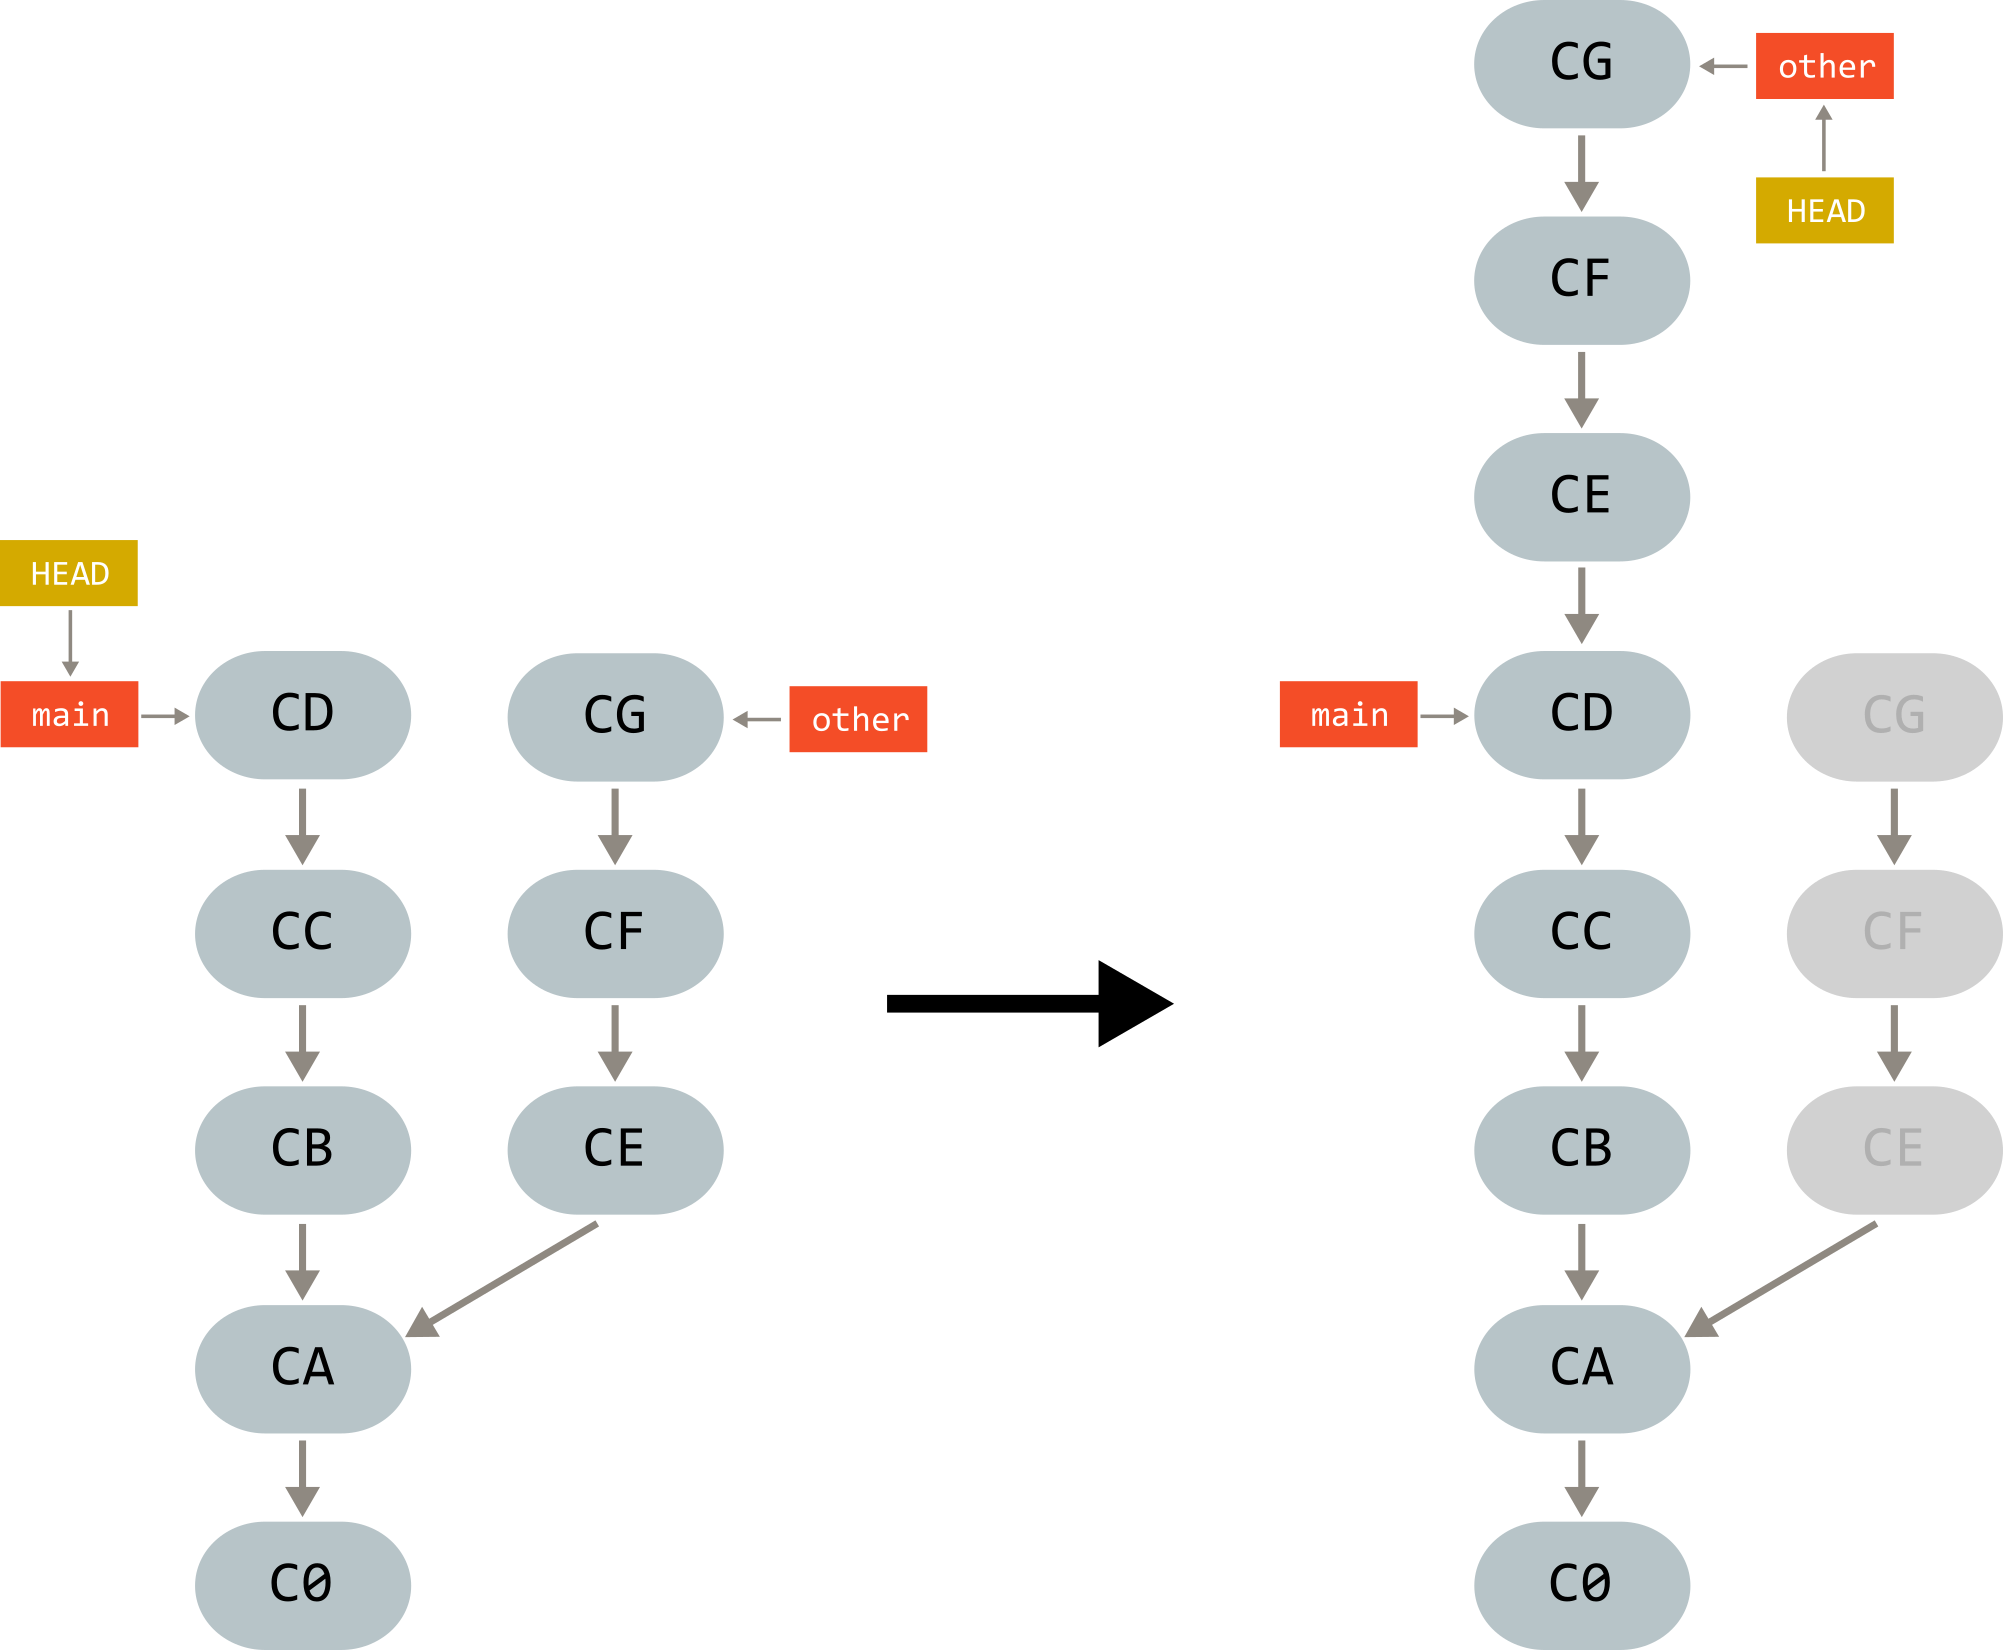
\includegraphics[scale=0.8]{../images/branch_animals_rebase.png}
\end{center}

\noindent Однако потом передумали и хотите отменить перебазирование. Напишите команды \texttt{git}, которые бы отменяли перебазирование и возвращали бы всё как прежде.

\subsection{Отмена \texttt{push}}
Для этой задачи вам нужно:
\begin{enumerate}
\item Создать новый локальный репозиторий на вашем компьютере с помощью скрипта \texttt{create\_animals.sh}.
\item Создать новый пустой репозиторий на GitLab.
\item Скопировать ссылку на GitLab репозиторий (протокол SSH).
\item Добавить новый remote на вашем локальном репозитории. 
\begin{lstlisting}[style=csMiptBash]
$ git remote add имя ссылка
\end{lstlisting}
Имя можно выбрать любое, но часто выбирают \texttt{origin}.
\item Проверьте, что новый remote добавился:
\begin{lstlisting}[style=csMiptBash]
$ git remote -v
\end{lstlisting}
\item Отправьте ваш локальный репозиторий на GitLab.
\begin{lstlisting}[style=csMiptBash]
$ git push -u origin main
\end{lstlisting}
\end{enumerate}

\noindent Предположим, что вы создали новый файл и добавили его в область индексирования, в локальный репозиторий, а затем и в улалённый репозиторий.
\begin{lstlisting}[style=csMiptBash]
$ touch emu.txt
$ git add emu.txt
$ git commit -m "add emu.txt"
$ git push
\end{lstlisting}
Однако затем передумали и хотите отменить коммит. Вы хотите, чтобы изменения пропали везде -- как на вашем компьютере, так и в последнем состоянии удалённого репозитория. Решите эту задачу двумя способами:
\begin{itemize}
\item Используя \texttt{git push}.
\item Используя \texttt{git revert}.
\end{itemize}


\end{document}
